% !Mode:: "TeX:UTF-8"
\chapter{分支预测器介绍}


本章首先介绍香山处理器第二版分支预测的整体架构,各个预测器在流水级中的先后关系和联系。其次针对每个预测器都介绍了它们的预测原理和功能。并指出它们相对于第一版设计做出的修改,以及做出相关修改的原因。

\section{分支预测整体结构}

香山第二版分支预测架构采用的是4级流水设计,架构图如图2.1所示。在4个流水级中,S0主要负责收集S1、S2、S3流水级的预测结果,以及取指单元和流水线后端发挥的分支误预测信息,从中选择出下一周期需要进行预测的pc,然后将该pc对应的读请求发给各个预测器,不同的预测器得出预测结果的时间需要1到2周期不等。

香山分支预测的主要预测器使用的是TAGE算法,但是由于更加准确的预测器得出预测结果需要的时间更久,超过了一个周期所需的时间,为了能够让分支预测流水线无气泡的流水,因此首先需要一个每周期都能够做出一次预测结果的预测器,也就是负责在S1做出预测的Micro BTB,它每周期都能够针对上一个周期的pc给出预测结果,及时的给出下一周期需要预测的pc,这样就能够让流水线无气泡的工作。之后S2是由FTB、TAGE和RAS联合做出的预测结果,由于S2的算法更复杂,能够覆盖更多的情况,因此我们认为它的预测准确率高于S1。当出现S2的预测跳转方向和跳转目标地址和S1预测的结果不相同时,我们会以S2的预测结果为准,这意味着之前S1预测的结果需要修正,需要清空S2之前的流水线,从S2预测的下一周期目标地址开始重新预测,这时分支预测流水线就会产生1拍的气泡。同样的,在S3会使用SC和ITTAGE再进行一次预测, 我们认为这次的预测是最准确的,也就是说S2的预测结果和S3预测结果不同时以S3的结果为准。当出现S2和S3预测结果不同时,也需要刷新分支预测流水线重新取指,这会带来2周期的气泡。

相比于第一版的设计,第二版最重要的一个改动就是将取指功能和分支预测部分解耦,我们将分支预测流水线和取指流水线统一称为前端流水线,而在这之后的流水线称为后端流水线。通过重构前端,我们将取指部件的执行顺序移到了分支预测之后,这样做的好处在于可以减少一些前端流水线的气泡。

\begin{figure}[htb]
	\centering
	\setlength\tabcolsep{3pt}  % 同一行中的图片间隔
	\vspace{5pt} % 图片上部的空白,如果太小的话,图片顶部会与正文内容十分接近
	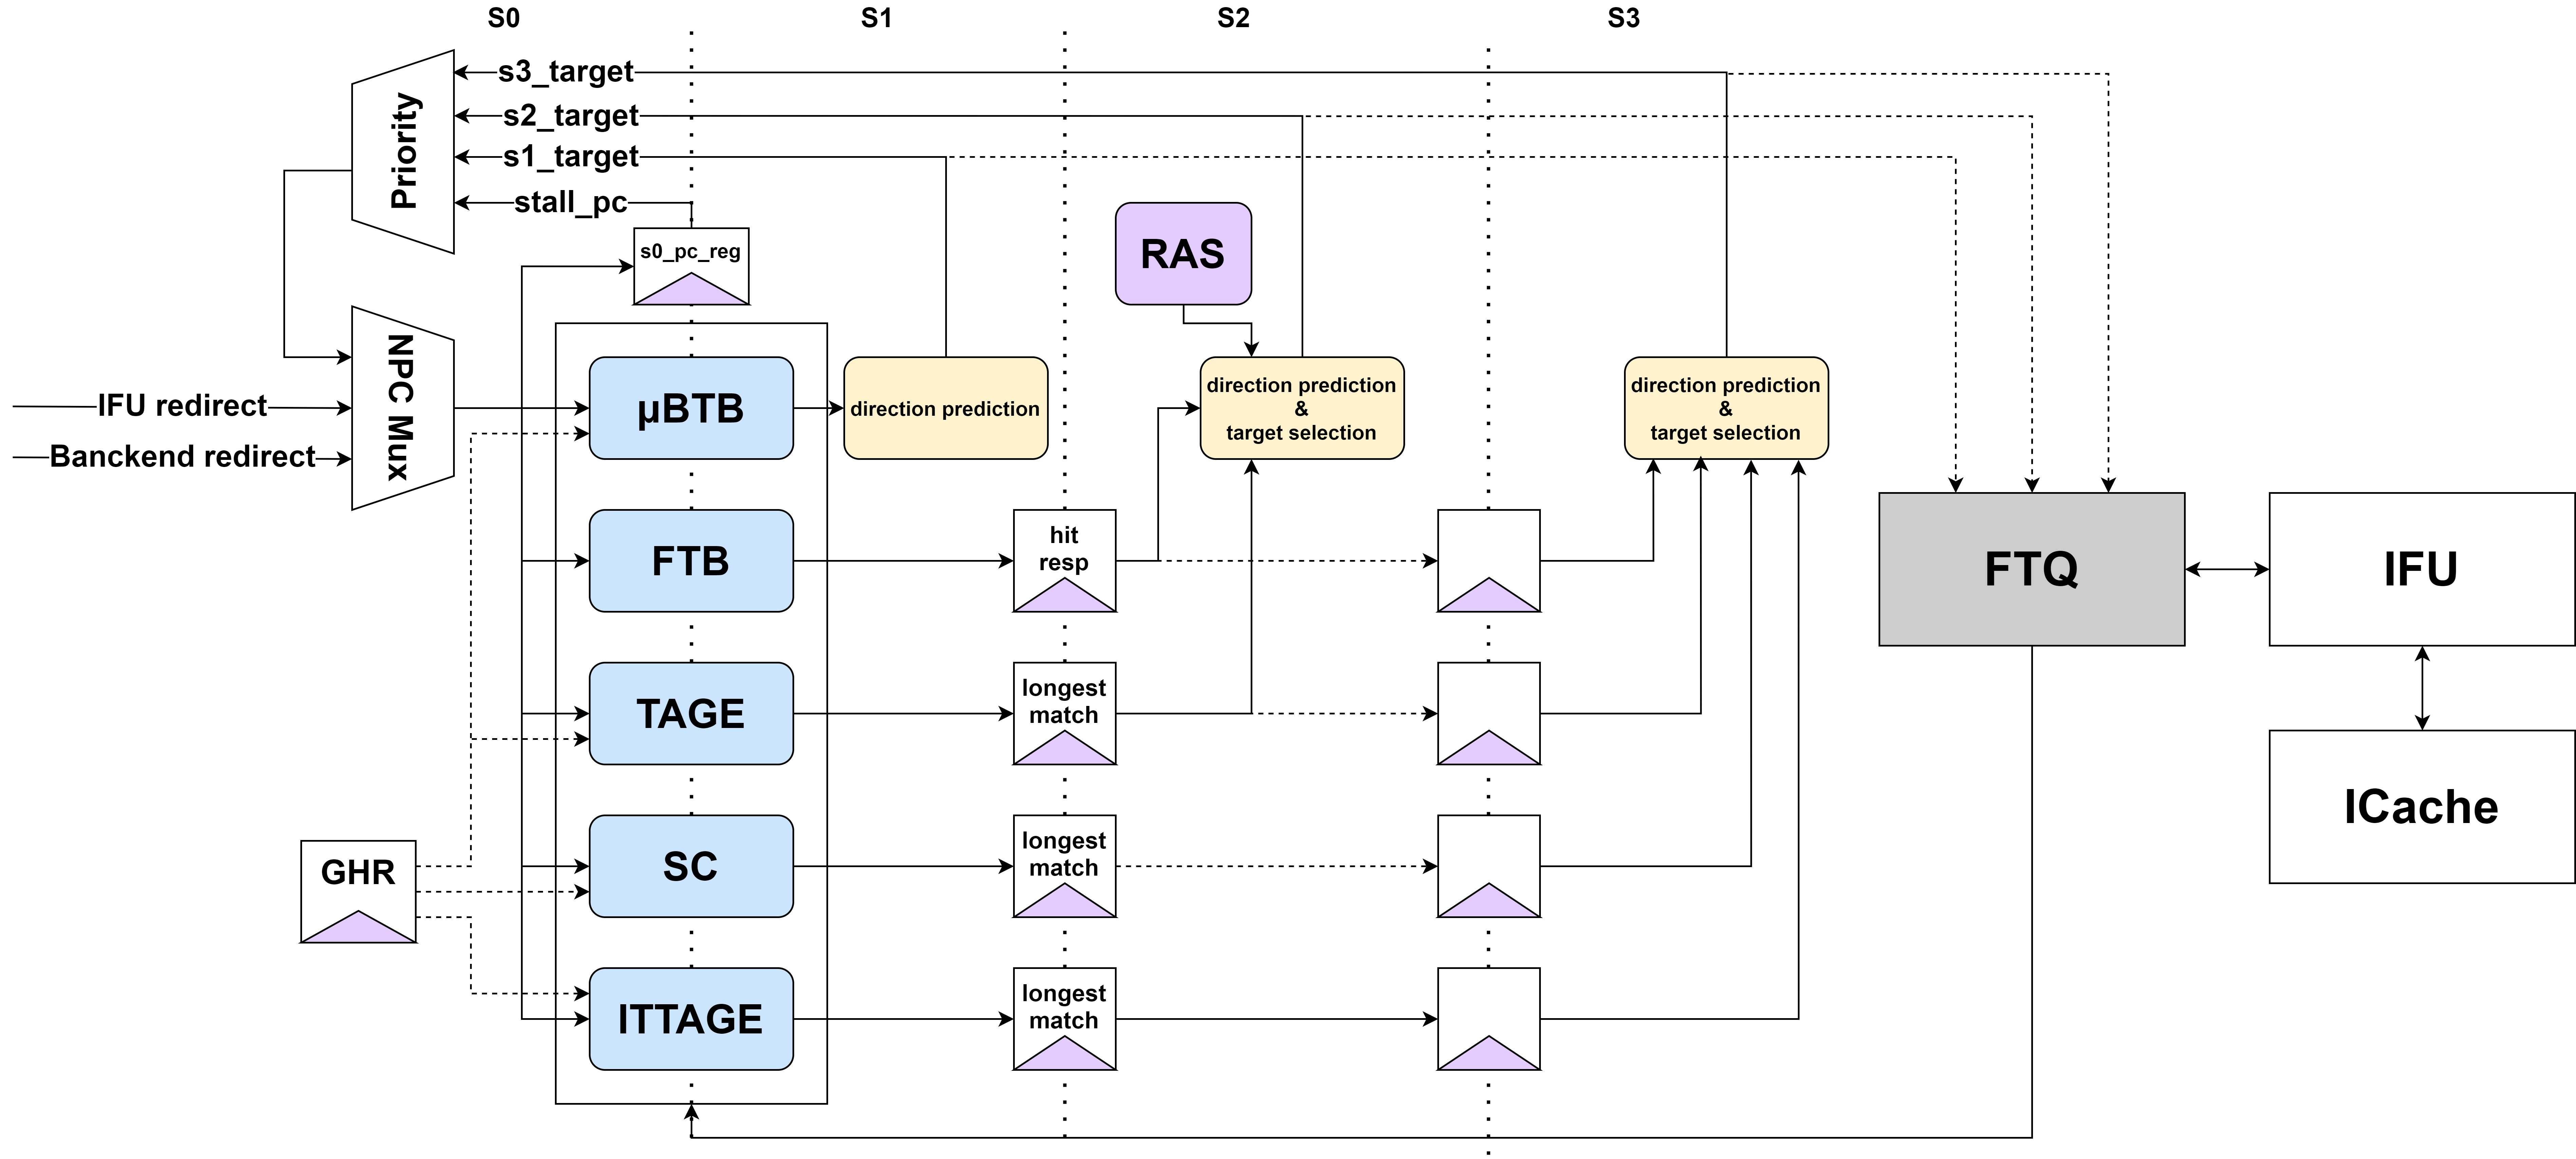
\includegraphics[width=1\textwidth]{BPU-FTQ-IFU.jpg}
	\caption{香山处理器第二版分支预测架构图}
	\label{fig:figure1}
\end{figure}

\section{FTB设计介绍}

由于分支预测通常运行在取指之前,因此我们无法通过对指令码进行预译码来识别一条指令是否是分支指令,也无法知道一条分支指令的跳转目标地址。即使在第一版的设计中,取指和分支预测同时进行,等到将指令码从指令缓存中取回时,也要等到2周期以后。因此我们需要在分支指令执行完毕时将它们保存在一个buffer中,通过它们的pc进行索引,这样下次再遇到同一条分支指令时,我们就可以通过查找这个buffer来获得它的相关信息,从而得知它的指令类型和跳转目标地址。这就是BTB (Branch Target Buffer) 的主要功能。它负责在预测时指出哪些指令是分支指令,以及它们对应的跳转目标地址。

在第一版设计中的BTB,以单条分支指令为基本单位,而由于我们前端的取指宽度是32Byte,算上4Byte长的普通指令和2Byte的压缩指令,一次取指中最多可能同时有16条分支,即16条都是压缩指令的情况,因此第一版设计中的BTB总共有16个bank,每个bank对应指令块中可能是一条分支指令的起始位置。而相对的我们进行分支预测时,也要同时对这16条指令进行索引和预测,再最后我们要从这16条预测结果中选出最终生效的一条指令,将其预测的下一周期取指pc送回S0。

在第二版的设计中,为了减少分支预测宽度,降低流水级中的逻辑门级数,我们采用了Glenn提出的FTB (Fetch Target Buffer) 设计,相比于BTB,FTB主要的改变在于将buffer中储存的项由单条分支修改为了一个有一定约束的取指块 (Fetch Block,注:不同于编译原理里的Fetch Block),通过给定的约束,前端每次的取指宽度由32Byte的固定大小改为了不固定的大小,每个Fetch Block的大小由block中分支指令的分布决定,Fetch Block限制了每个block中分支指令的数量上限,在第二版设计中,我们限制每个block中最多只能够有2条条件分支指令 (branch)和一条无条件跳转指令 (jump)。通过这种设计,我们能够将分支预测的宽度由第一版的16降低为2,从而减少最后的选择逻辑门级数,达到减少组合逻辑电路延迟的效果。

\section{Micro BTB设计介绍}

Micro BTB作为一个小型的预测器,需要在每周期内都得出一个初步的预测结果,来保证分支预测流水线的连续。因此首先具有一个小型FTB的功能,它也能够保存分支指令的信息,但是由于它需要在很快的时间内做出一个初步的预测,因此它的逻辑必须简单,使用的硬件资源必须足够小,因为过于复杂的逻辑和过多的面积都会导致它无法按时给出预测结果。

在第一版的设计中,Micro BTB就是一个小型的BIM和BTB的集合体,它使用自己的存储空间存储了少量的分支指令信息,并且有自己单独的一组两位饱和计数器,通过索引分支指令信息,并且以两位饱和计数器的值来给出预测结果。

在第二版的设计中,由于需要满足更高的频率要求,修改了Micro BTB的预测算法,首先使用要预测的pc和全局历史哈希做索引,当Micro BTB命中,即发现当前pc对应的取指块已经被保存时,它会依据上一次索引到该项的分支的跳转方向,以此作为这次的预测结果。这种逻辑会比更新和计算饱和计数器更加简单,同时不会有太大的性能损失。

\section{RAS设计介绍}

RAS (Return Address Stack) 是一个专门针对call和return指令优化的预测器。我们知道通常程序执行某个函数时,首先会使用一条call指令跳转到函数的起始地址,然后函数的最后会有一条return指令,再将程序跳转回call指令之后的下一条指令继续执行。由于函数调用是递归的,因此可以使用一个栈结构来保存所有函数调用的返回地址。当检测到一条call指令时,将这条call指令之后的下一条指令存入RAS,然后当检测到一条return指令时,就将RAS栈顶保存的地址出栈,作为这条return指令的跳转目标地址。

由于程序中有大量的类似于递归调用的行为,因此我们的每个RAS项都带有一个计数器,当连续的几次调用都相同时,我们只有第一条call指令会调用入栈操作,之后的call指令只会不断增加栈顶元素的计数器。同样的在return指令时,首先会检测栈顶元素的计数器,如果计数器大于1,则不弹出栈顶元素,只是将栈顶元素的计数器减1,直到计数器为1时才出栈。

而为了减少预测时读取RAS的延迟,我们另外使用了一个专门的寄存器用来存储当前栈顶的地址副本,当我们检测到一条return指令时,就可以直接使用这个单独的寄存器,而不用从整个RAS栈中读取栈顶元素。

RAS在分支指令出现误预测时需要恢复,不然可能会出现地址错乱的情况,而我们使用了一种较为简单的恢复方法,即在分支预测时将当前的栈顶指针和栈顶元素保存起来,在恢复时只恢复栈顶元素和指针,这样一来既能够简化恢复逻辑,也不会带来过多的误预测。

\section{TAGE设计介绍}

TAGE (TAgged GEometric history length branhc predictor) 是在2004年第一件分支预测大赛上由André提出的一种预测器,之后不断地优化和改进,多次夺得了分支预测大赛的冠军,也是目前公开的分支预测性能最好的预测器。TAGE是一个使用全局历史索引的方向预测器,也就是说它只会用来预测分支是否跳转,而跳转目标地址需要由FTB、RAS或ITTAGE来提供。
TAGE由多张预测表组成,每张表通过不同长度的分支历史来索引,表中的每一项都是一个饱和计数器。每次预测时会同时查找所有的表,然后从中选择出历史长度最长且tag匹配的表,以它的饱和计数器值作为分支预测的结果。

\section{SC设计介绍}

SC (statistical corrector) 是TAGE预测器的一个组件,用来预测一部分TAGE不能准确预测的分支指令,即与全局历史没有太多相关性,但是跳转方向有明显的偏向值的分支。

\section{ITTAGE设计介绍}

ITTAGE (Indirect Target TAgged GEometric history length branhc predictor) 是一个专门针对间接跳转分支的预测器,其算法大部分与TAGE相同。不同之处在于TAGE中用于判断跳转方向的饱和计数器被替换成了一个跳转目标地址和一个置信度计数器

\section{本章小结}

本章主要详细介绍了本文提出的分支预测架构的流水线设计和工作流程,单独列出了多个预测器的功能和算法